\section{Forces on a 2-dimensional body}

With the Bernoulli equation, 
\begin{equation}
\vec{\nabla}\left(\frac{\rho}{2}\vec{u}^2+p\right)=0.
\end{equation}
we can calculate the force on the "obstacle" (\fref{fig:2dim-body}) from the surrounding flow:
\begin{align}
\vec{F} &= \int_{S}(-p(\vec{r}))d\vec{A} = -\int_{S}\left(p_0-\frac{\rho}{2}\vec{u}^2(\vec{r})\right)d\vec{A} \\
&= \frac{\rho}{2}\int_{S}\vec{u}^2(\vec{r})d\vec{A}\\
&= L\vec{e}_y +\underbrace{D\vec{e}_x}_{=0}.
\end{align}
$\vec{L}$ is the lift force and $\vec{D}$ is the drag force. The last term equals zero because there is no friction in ideal flows.

\begin{figure}[!h]
    \centering
    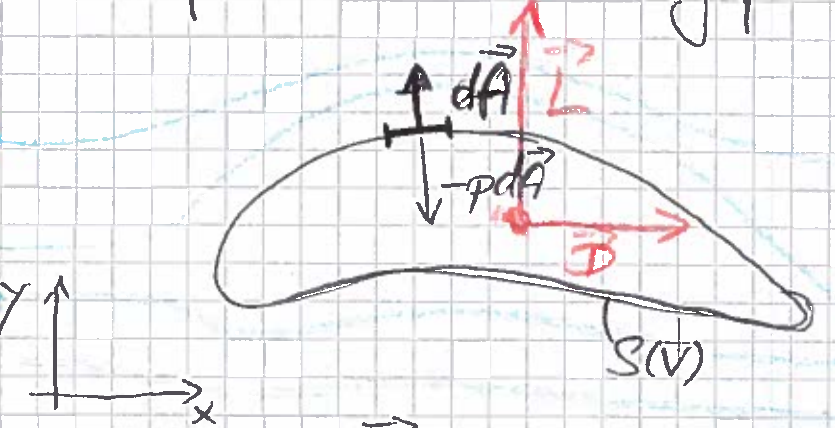
\includegraphics[width=.5\textwidth]{week4/2dim-body}\\
    \caption{Lift and drag forces.}
    \label{fig:2dim-body}
\end{figure}

\begin{figure}[!h]
    \centering
    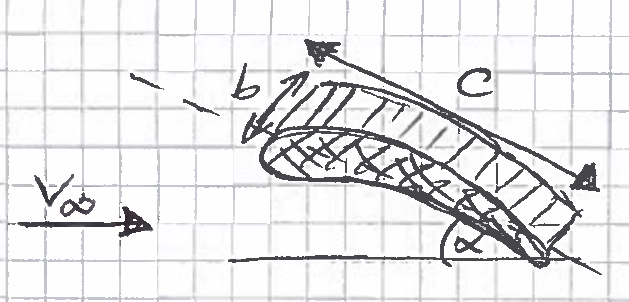
\includegraphics[width=.4\textwidth]{week4/generic-lift2}\\
    \caption{Angle of attack.}
    \label{fig:generic-lift2}
\end{figure}

Lift coefficient
\begin{equation}
C_L = \frac{L}{\frac{\rho}{2}v_\infty^2 b c}
\end{equation}
Drag coefficient (for the case that friction is non-zero):
\begin{equation}
C_D = \frac{D}{\frac{\rho}{2}v_\infty^2 b c}
\end{equation}

\begin{figure}[!h]
    \centering
    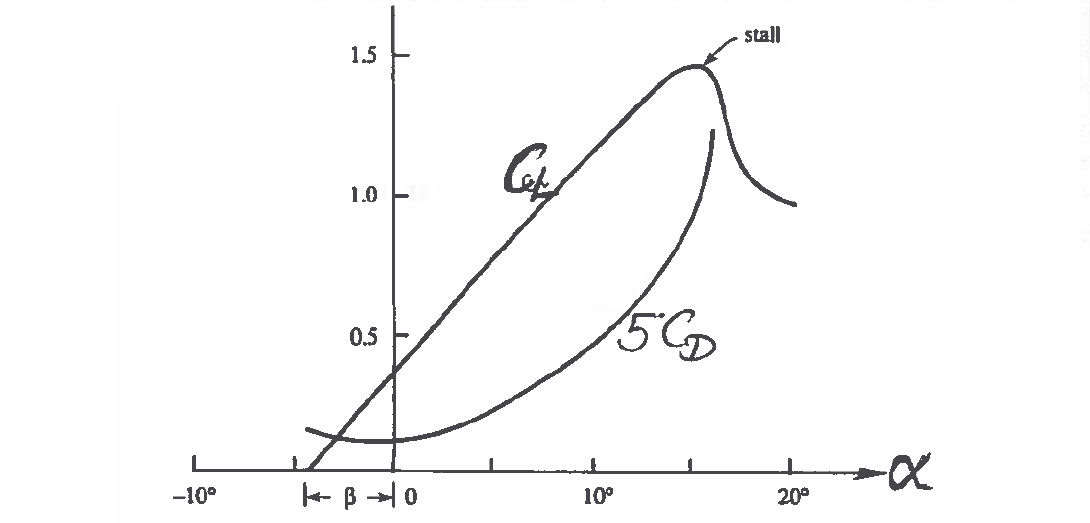
\includegraphics[width=.5\textwidth]{week4/generic-lift}\\
    \caption{Generic lift and drag coefficients vs. angle of attack.}
    \label{fig:generic-lift}
\end{figure}


\subsection{Turbine blade}
The lift force pulls the rotor blade of a wind turbine forward. See \fref{fig:turbine-blade}.
\begin{figure}[!h]
    \centering
    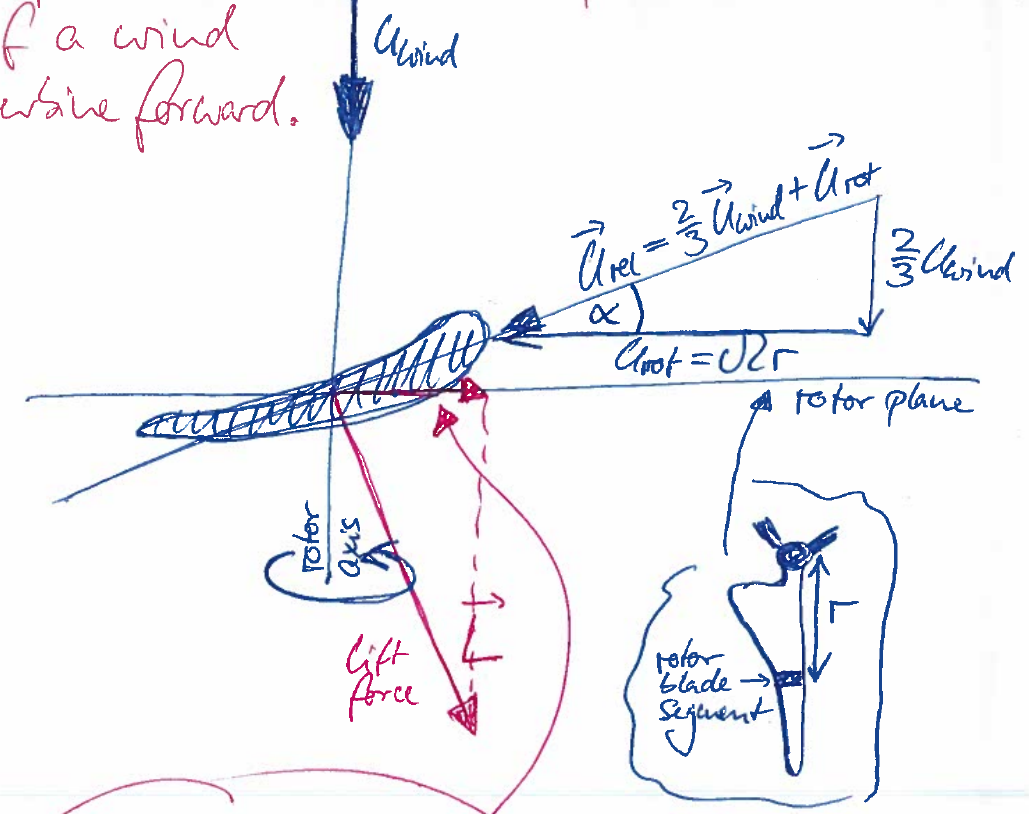
\includegraphics[width=.6\textwidth]{week4/turbine-blade}\\
    \caption{Lift force on the rotor blade of a wind turbine.}
    \label{fig:turbine-blade}
\end{figure}


\subsection[Sailing against the wind]{Sailing against the wind (KCD 14.9)}
People have sailed without the aid of an engine for thousands of years and have known
how to reach an upwind destination. Actually, it is not possible to sail exactly against the
wind, but it is possible to sail at $\approx$ 40-45$^\circ$ to the wind. \fref{fig:sailing-wind} shows
how this is made possible by the aerodynamic lift on the sail, which is a piece of stretched and stiffened
cloth. The wind speed is U, and the sailing speed is V, so that the apparent wind speed relative
to the boat is $U_r$. If the sail is properly oriented, this gives rise to a lift force perpendicular
to U$_\text{r}$ and a drag force parallel to U$_\text{r}$. The resultant force F can be resolved into a driving
component (thrust) along the motion of the boat and a lateral component. The driving
component performs work in moving the boat; most of this work goes into overcoming
the frictional drag and in generating the gravity waves that radiate outward from the hull.
The lateral component does not cause much sideways drift because of the shape of the
hull. It is clear that the thrust decreases as the angle $\theta$ decreases and normally vanishes
when $\theta$ is $\approx$ 40-45$^\circ$ . The energy for sailing comes from the wind field, which loses kinetic
energy after passing the sail.

\begin{figure}[!h]
    \centering
    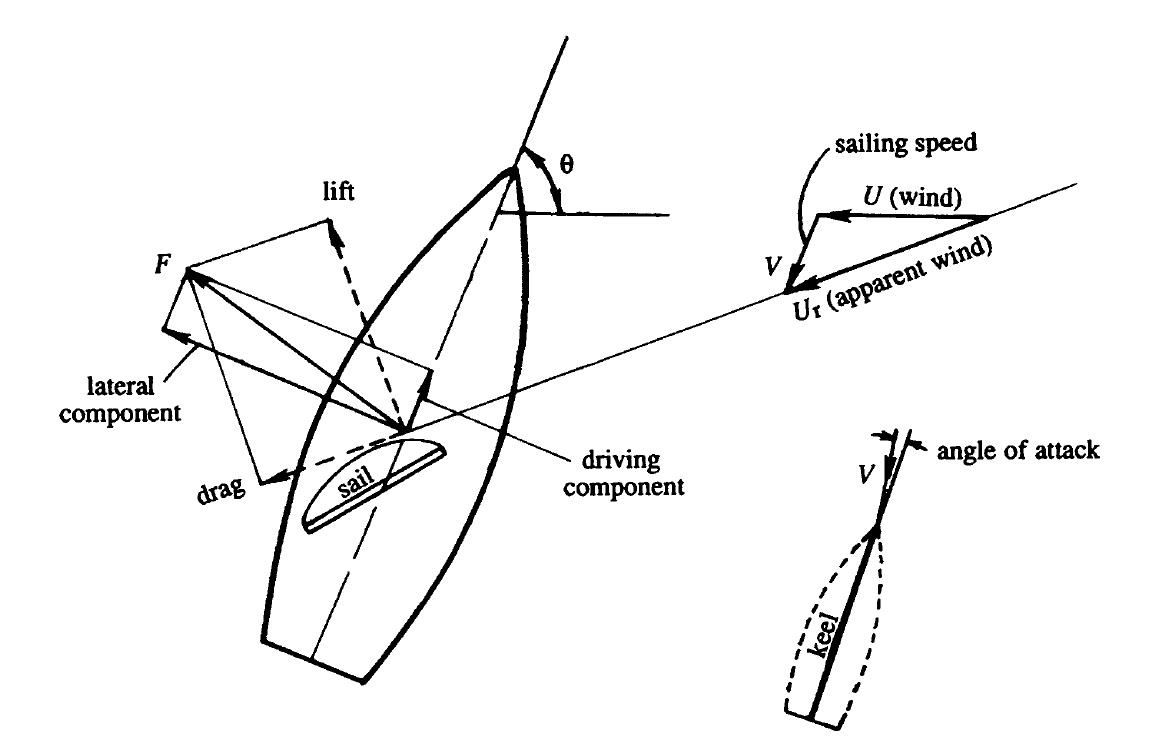
\includegraphics[width=.6\textwidth]{week4/sailing-wind}\\
    \caption{Principle of sailing against the wind. A small component of the sail’s lift pushes the boat forward at an angle $\theta$ < 90$^\circ$ to the wind. Thus by traversing a zig-zag course at angles $\pm\theta$, a sailboat can reach an upwind destination. A sailboat’s keel may make a contribution to its upwind progress too.}
    \label{fig:sailing-wind}
\end{figure}

\newpage
\subsection{Reynolds number}
Fluid around a cylinder can create several real flow patterns. See \fref{fig:reynolds-cylinder}.

\begin{figure}[p]
    \centering
    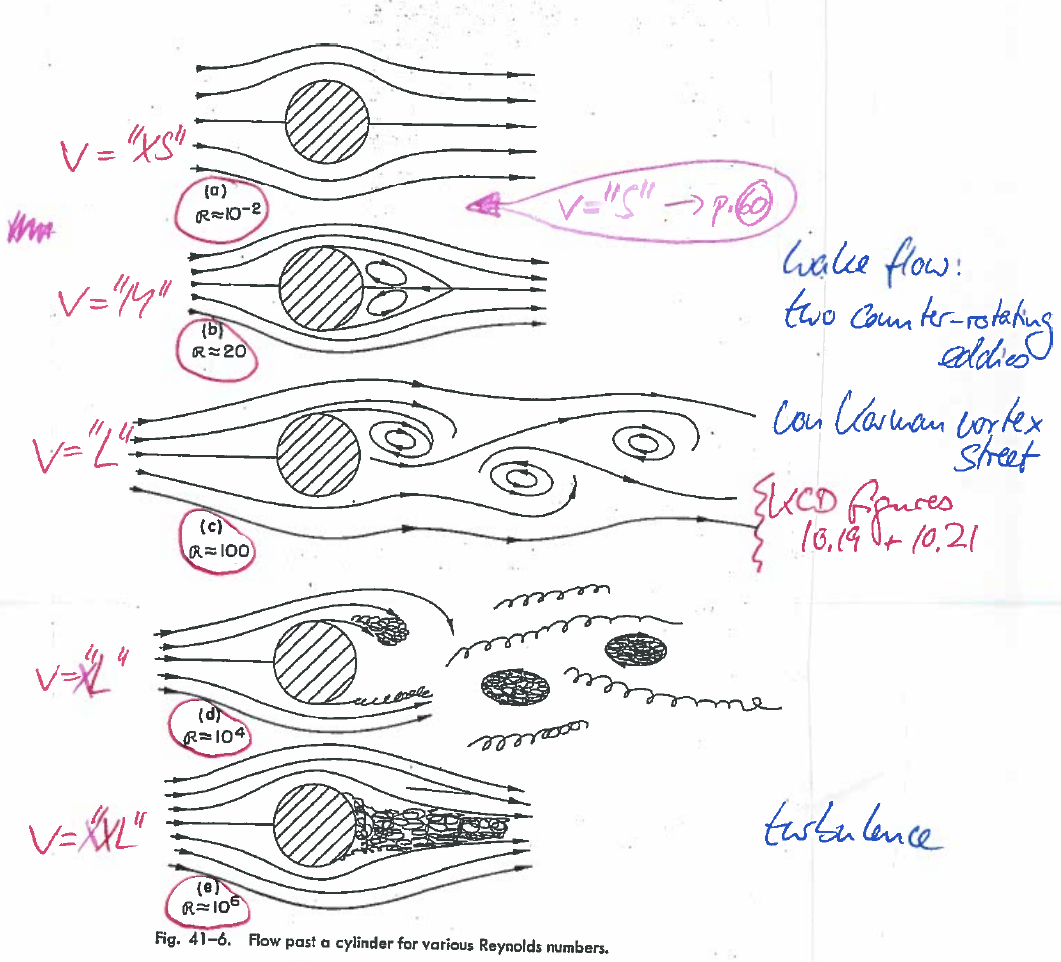
\includegraphics[width=\textwidth]{week4/reynolds-cylinder}\\
    \caption{Flow around a cylinder. From laminar to turbulent with increasing velocity.}
    \label{fig:reynolds-cylinder}
\end{figure}

\textbf{Questions:}
\begin{enumerate}
\item Why so many different flows?
\item What causes and characterizes them?
\end{enumerate}
Certainly friction, i.e. viscosity, will have something to do with it.

\begin{align}
0 &= \rho_0 \left[\pdiff{\vec{u}}{t}+\left(\vec{u}\cdot\vec{\nabla}\right)\vec{u}\right] + \vec{\nabla}p - \mu \left(\vec{\nabla}\cdot\vec{\nabla}\right) \vec{u} \\
&= \rho_0\left[\frac{U}{T}\pdiff{\vec{u}'}{t'}+\frac{U^2}{L}\left(\vec{u}'\cdot\vec{\nabla}'\right)\vec{u}'\right] + \frac{\rho_0 U^2}{L}\vec{\nabla}'p'-\mu\frac{U}{L^2}\left(\vec{\nabla}\cdot\vec{\nabla}\right)'\vec{u}' \\
&= \rho_0\frac{U^2}{L} \left\lbrace \pdiff{\vec{u}'}{t'}+\left(\vec{u}'\cdot\vec{\nabla}'\right)\vec{u}'+\vec{\nabla}'p'-\frac{\mu}{\rho_0 LV} \left(\vec{\nabla}\cdot\vec{\nabla}\right)'\vec{u}' \right\rbrace
\end{align}
where $L$ is the characteristic length, $U$ is the characteristic velocity, $T=L/U$ is the characteristic time, and $P=\rho_0U^2$ the characteristic pressure.

Reynolds number:
\begin{equation}
Re = \frac{\rho_0 L U}{\mu}
\end{equation}

\begin{framed}
\textbf{Remark:} law of similarity

If two flows have the same geometry (object) and the same Reynolds number, but a different absolute scale it means that the two flows are similar (identical, except for a scale transformation). Applications of this is wind tunnel experiments of air wings, wind turbine blades, cars, etc.
\end{framed}

The Reynolds number
\begin{equation}
Re = \frac{\rho_0 L U}{\mu} = \frac{\rho_0 U^2/L}{\mu U/L},
\end{equation}
is the inertia force density divided by the friction force density.

\begin{figure}[p]
    \centering
    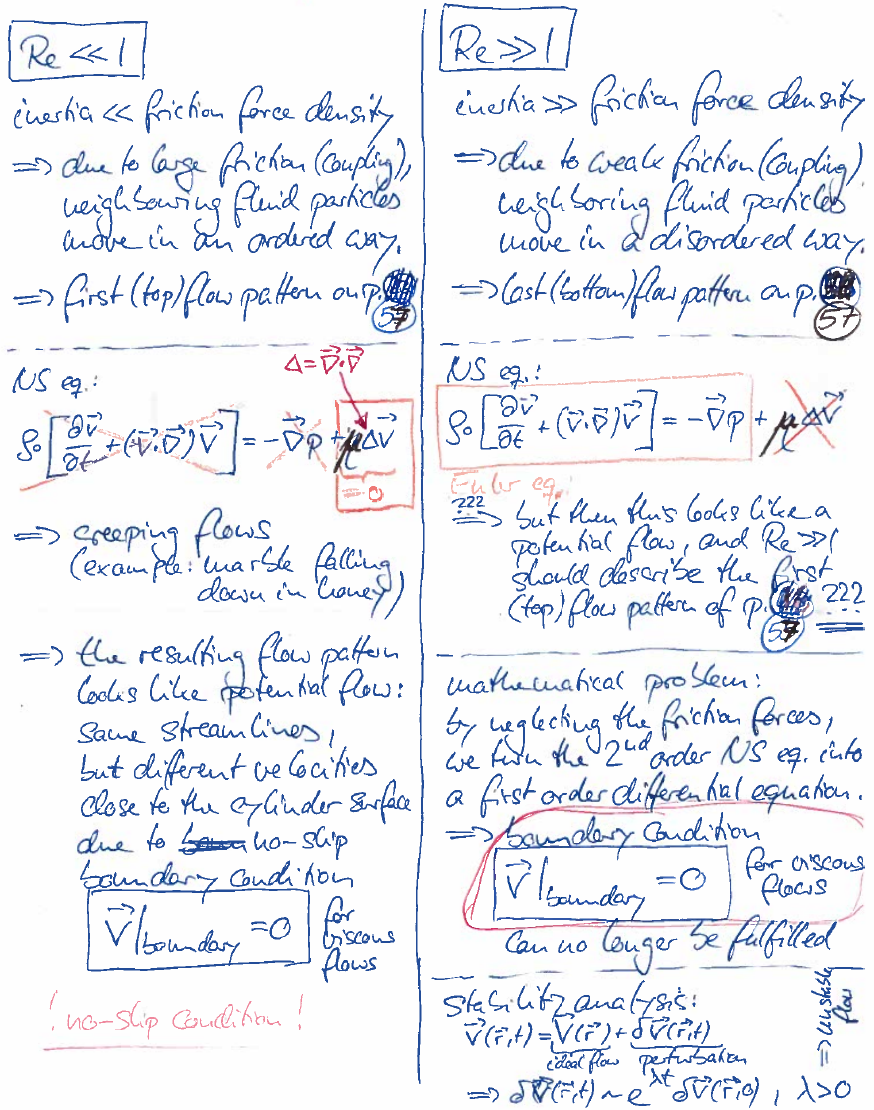
\includegraphics[width=\textwidth]{week4/reynolds-numbers}\\
    \caption{Extreme examples of Reynolds number.}
    \label{fig:reynolds-numbers}
\end{figure}

\begin{figure}[p]
    \centering
    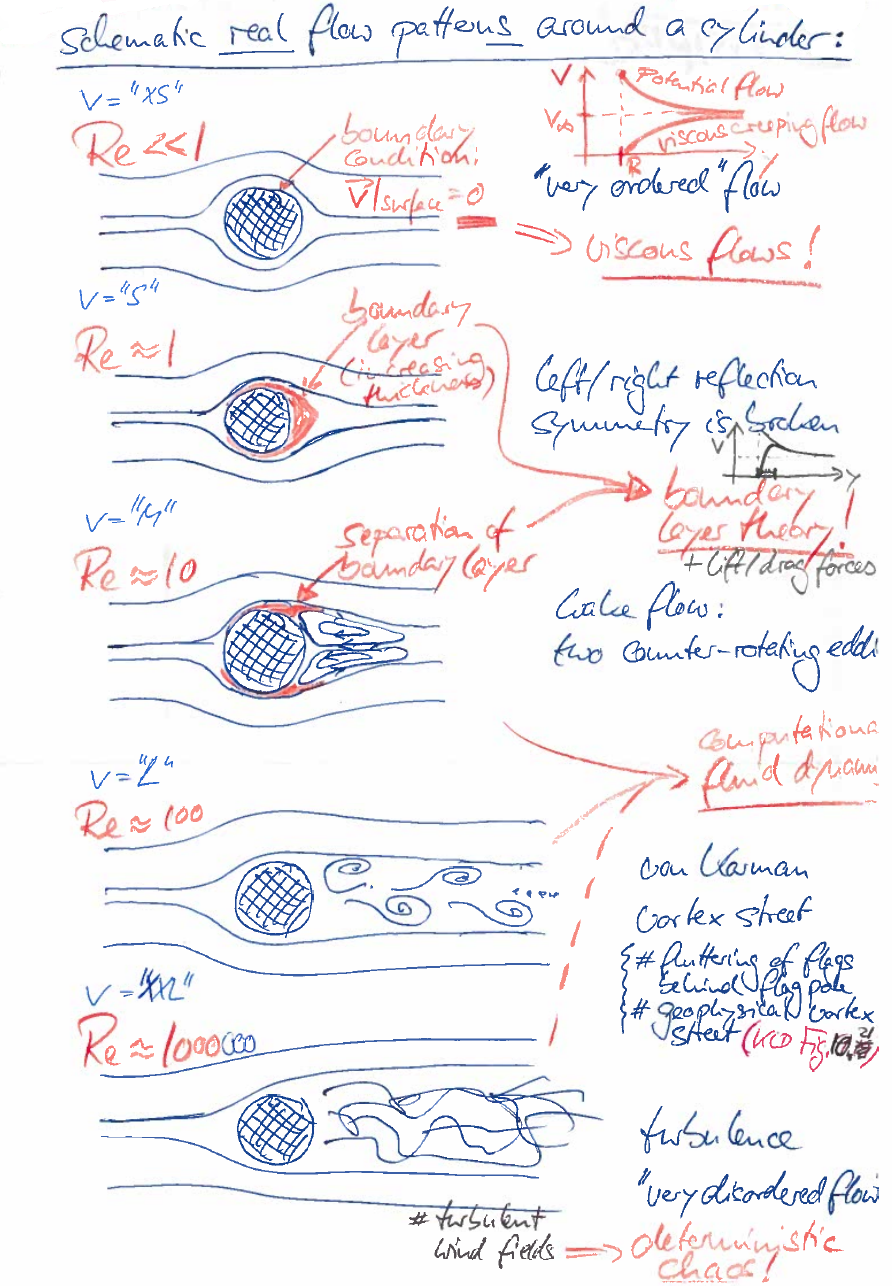
\includegraphics[width=\textwidth]{week4/schematic-flows}\\
    \caption{Schematic real flow patterns around a cylinder with different Reynolds numbers.}
    \label{fig:schematic-flows}
\end{figure}


\newpage
\subsection{Viscous pipe flow}

\begin{figure}[ht]
    \centering
    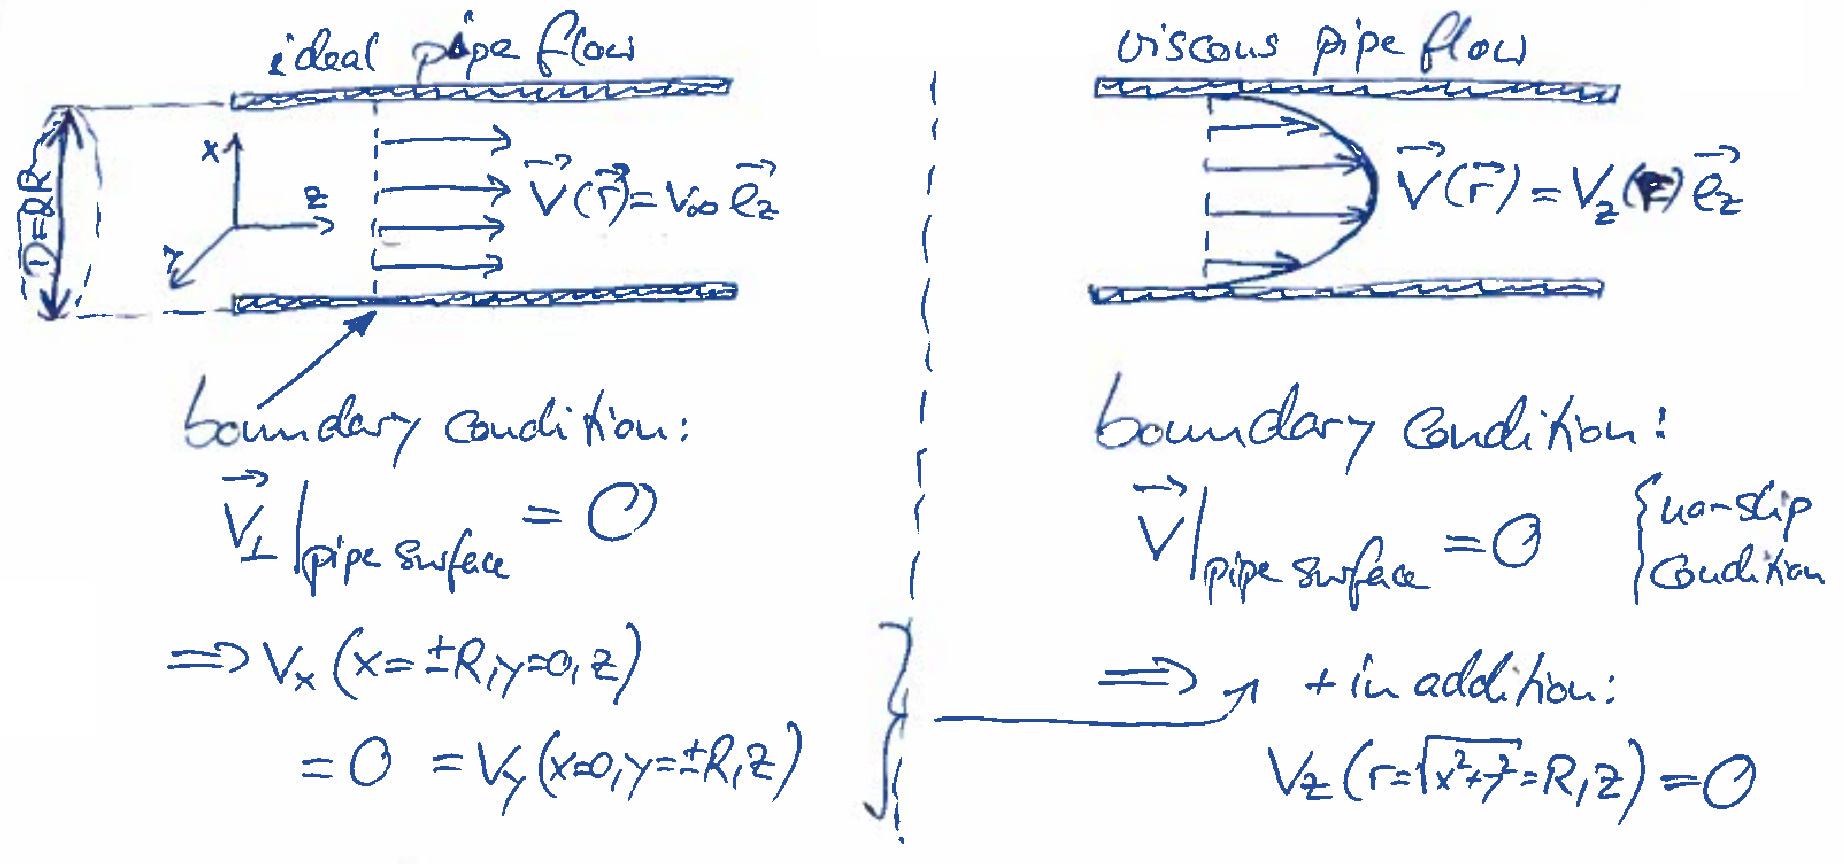
\includegraphics[width=\textwidth]{week4/viscous-pipe-flow}\\
    \caption{Ideal and viscous pipe flow.}
    \label{fig:viscous-pipe-flow}
\end{figure}

Task: calculate velocity profile $u_z=u_z(r)$ for the viscous pipe flow.

Navier-Stokes equation
\begin{equation}
\rho_0\underbrace{\pdiff{\vec{u}}{t}}_{=0}+\rho_0\underbrace{\left(\vec{u}\cdot\vec{\nabla}\right)}_{=0}\vec{u} = \underbrace{\vec{f}_\mathrm{ext}}_{=0}-\vec{\nabla}p+\mu\left(\vec{\nabla}\cdot\vec{\nabla}\right)\vec{u}
\end{equation}
The second term on the left-hand side vanishes because of the incompressibility condition
\begin{equation}
0=\vec{\nabla}\cdot\vec{u}=\partial_xu_x+\partial_yu_y+\partial_zu_z = \partial_zu_z
\end{equation}
with $u_x=u_y=0$ and
\begin{equation}
\left(\vec{u}\cdot\vec{\nabla}\right)\vec{u} = u_z\partial_z
\begin{pmatrix}
0\\0\\u_z
\end{pmatrix} = 0.
\end{equation}
\begin{align}
\vec{\nabla}p = \mu\left(\ppdiff{}{x}+\ppdiff{}{y}\right)u_z\vec{e}_z\\
\leadsto
\left(\vec{\nabla}p\right)_x &= \left(\vec{\nabla}p\right)_y = 0 \\
\leadsto
p &= p(z)
\end{align}

\begin{align}
\mu\left(\partial_x^2+\partial_y^2\right) v_z(r) &= \frac{\mu}{r}\pdiff{}{r}\left(r\pdiff{u_z(r)}{r}\right) \\
&= \pdiff{p(z)}{z} \require \mathrm{constant}
\end{align}

\begin{align}
\pdiff{p(z)}{z}&=c \\
\leadsto
p(z) &= cz+d \\
&= \frac{p(z=L)-p(z=0)}{L}z+p(z=0)\\
&= -\frac{\Delta p}{L}z + p(z=0)
\end{align}

\begin{align}
\frac{\mu}{r}\pdiff{}{r}\left(r\pdiff{u_z(r)}{r}\right) &= c = -\frac{\Delta p}{L} \\
\leadsto
r\pdiff{u_z(r)}{r} &= -\frac{\Delta p}{\mu L}\frac{r^2}{2} + D_1 \\
\leadsto
u_z(r) &= -\frac{\Delta p}{4\mu L}r^2 + D_1 \ln r + D_ 2 \\
\end{align}
$D_1$ and $D_2$ are determined from the boudnary conditions $u_z(r=R)=0$ (no slip condition) and $|u_z(r=0)|<\infty$ (finiteness).
\begin{equation}
u_z(r) = \frac{\Delta p}{4\mu L}\left( R^2 - r^2\right)
\end{equation}

Fluid mass per time passing through pipe cross-section:
\begin{equation}
\diff{M}{t} = \int_0^R\rho_0 u_z(r)2\pi r dr = \frac{\pi\rho_0 R^4\Delta p}{8\mu L}
\end{equation}
This is the Hagen-Poiseuille law.
\begin{framed}
\textbf{Remark:} this law allows to determine the viscosity:
\begin{equation}
\left\lbrace \underbrace{\rho_0,R,L}_\mathrm{known} \quad,\quad \underbrace{\Delta p,\diff{M}{t}}_\mathrm{measured} \right\rbrace \Rightarrow \mu
\end{equation}
\end{framed}

\begin{framed}
\textbf{Remark:} "Ohm's Law"

\begin{align}
\Delta p = \Delta U \ &,\quad \diff{M}{t} = I\\
\leadsto
I &= \frac{\pi\rho_0 R^4}{8L\mu} \Delta U
\end{align}

{\center
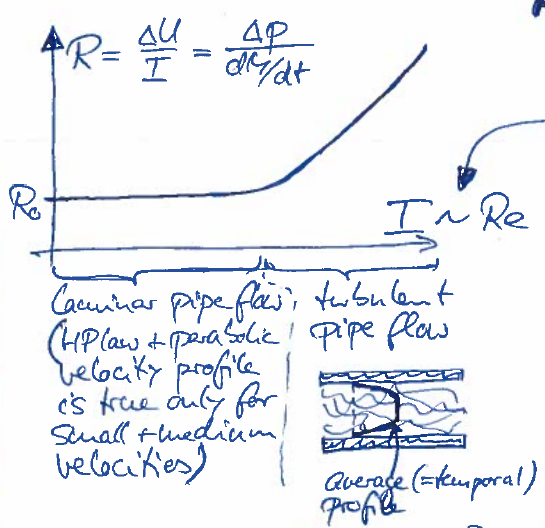
\includegraphics[width=.4\textwidth]{week4/ohms-law}\\
}

\begin{equation}
R = R_0\cdot f(Re)
\end{equation}
with
\begin{equation}
f(Re\rightarrow0)=1.
\end{equation}
Turbulence increases pipe resistance. This is important for the operation of oil and gas pipelines.
\end{framed}



\newpage
\subsection{Boundary layers}

\begin{figure}[ht]
    \centering
    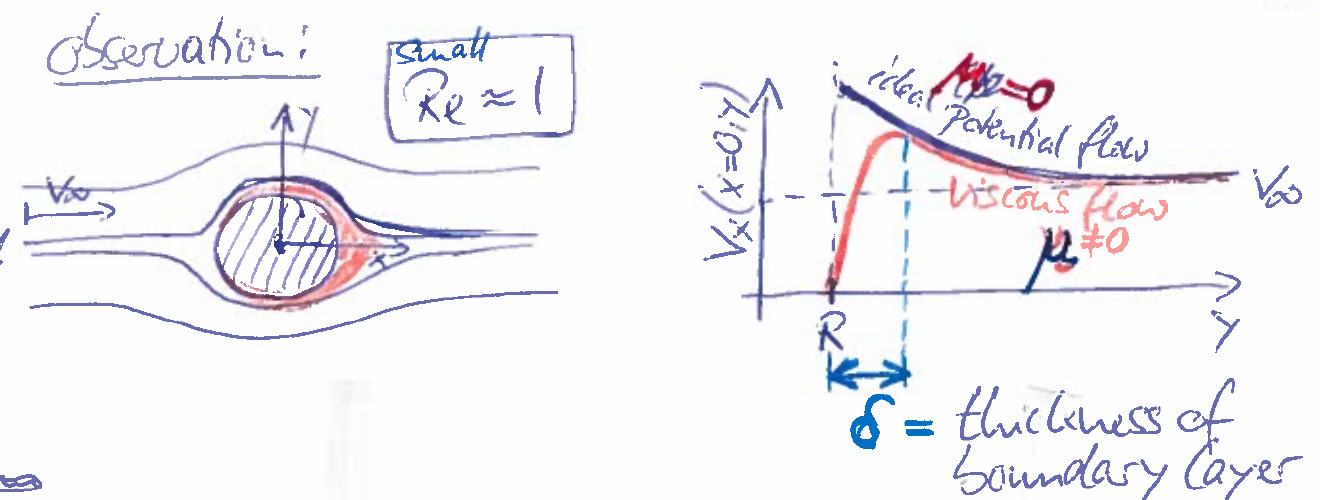
\includegraphics[width=\textwidth]{week4/boundary-layers}\\
    \caption{Example of boundary layer for flow around a cylinder.}
    \label{fig:boundary-layers}
\end{figure}

Idea of boundary layer theory:
\begin{enumerate}
\item within the boundary layer the velocity increases from zero to the ideal flow velocity
\item inside the boundary layer we use the Navier-Stokes equation (with friction)
\item outside the boundary layer we use the Euler equation without friction i.e. ideal potential flow
\item at the boundary surface we match the inside solution with the outside solution
\end{enumerate}

Derivation of the (laminar) boundary layer equations. Approximation to the Navier-Stokes equation inside the boundary layer. See \fref{fig:laminar-boundary}.

\begin{figure}[ht]
    \centering
    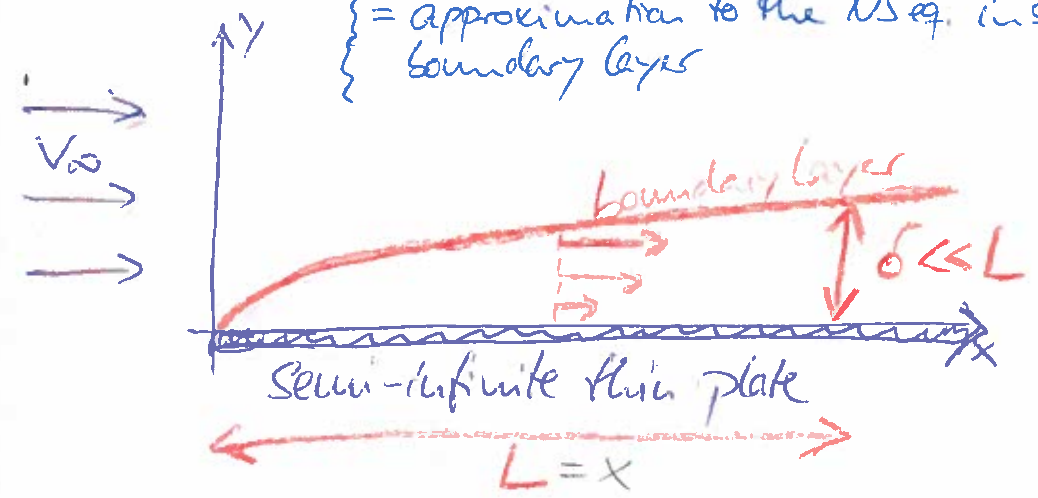
\includegraphics[width=.7\textwidth]{week4/laminar-boundary}\\
    \caption{Laminar boundary layer.}
    \label{fig:laminar-boundary}
\end{figure}

In the following we determine $\delta = \delta(x)$ (\fref{fig:laminar-boundary}) without solving the Navier-Stokes equation.

Incompressible flow:
\begin{align}
\vec{\nabla}\cdot\vec{u} = \pdiff{u_x}{x} + \pdiff{u_y}{y} &= 0 \\
\leadsto
\mathcal{O} \left(\frac{u_\infty}{L}\right) + \mathcal{O} \left(\frac{u_y}{\delta}\right) &= 0\\
\leadsto
\mathcal{O}(u_y) &= \delta\frac{u_\infty}{L} = \frac{\delta}{L}u_\infty
\end{align}

Navier-Stokes equation (x-component):
\begin{equation}
u_x\pdiff{u_x}{x} + u_y\pdiff{u_x}{y} = -\frac{1}{\rho_0}\pdiff{p}{x} + \frac{\mu}{\rho_0}\ppdiff{u_x}{x} + \frac{\mu}{\rho_0}\ppdiff{u_x}{y}
\end{equation}
\begin{equation}
\mathcal{O} \left(\frac{u_\infty^2}{L}\right) \require \mathcal{O} \left(\frac{\mu}{\rho_0}\frac{u_\infty}{\delta^2}\right)
\end{equation}

\begin{equation}
\left(\frac{\delta}{L}\right)^2 \sim \frac{\mu}{\rho_0 L u_\infty} = \frac{1}{Re}
\end{equation}
The larger the Reynolds number, the thinner the boundary layer. This holds for $Re \leq \SI{1e5}{}-\SI{1e6}{}$, above that the boundary layer becomes turbulent, and is no longer laminar.

\begin{equation}
\delta(x) \sim \sqrt{\frac{\mu x}{\rho_0 u_\infty}}
\end{equation}

Navier-Stokes equation (y-component):
\begin{equation}
u_x\pdiff{u_y}{x} + u_y\pdiff{u_y}{y} = -\frac{1}{\rho_0}\pdiff{p}{y} + \frac{\mu}{\rho_0}\ppdiff{u_y}{x} + \frac{\mu}{\rho_0}\ppdiff{u_y}{y}
\end{equation}
Ther first term on the right-hand side is the only large term. All other terms are neglected, which leads to
\begin{equation}
\pdiff{p}{y} = 0 \Rightarrow p = p(x)
\end{equation}

\begin{framed}
\textbf{Prandtl equations:} laminar boundary layer equations
\begin{align}
u_x\pdiff{u_x}{x}+u_y\pdiff{u_x}{y} &= -\frac{1}{\rho_0}\pdiff{p(x)}{x}+\frac{\mu}{\rho_0}\ppdiff{u_x}{y} \\
\pdiff{u_x}{x}+\pdiff{u_y}{y}&=0
\end{align}
\end{framed}

\textbf{Example:} Solution of Prandtl equations for laminar boundary flow around semi-infinite plate

\begin{equation}
p=p(x) \Rightarrow p(x)|_\mathrm{inside} = p(x)|_\mathrm{outside}
\end{equation}

Outside boundary layer:
\begin{align}
u_x|_\mathrm{outside} &= u_x = u_\infty = \mathrm{constant} \\
u_y|_\mathrm{outside} &= 0
\end{align}

Bernoulli equation:
\begin{align}
p(x) + \frac{\rho_0}{2}u_x^2 &= \mathrm{constant}\\
\leadsto
p(x) &= \mathrm{constant} \\
\leadsto
\pdiff{p(x)}{x} &= 0
\end{align}
Prandtl equations inside boundary layer:
\begin{align}
u_x\partial_xu_x+u_y\partial_yu_y &= \frac{\mu}{\rho_0}\partial_y^2u_x\\
\partial_xu_x+\partial_yu_y &= 0
\end{align}

\textbf{Solution:} similarity ansatz.
\begin{equation}
u_x(x,y) = u_\infty g\left(\frac{y}{\delta(x)}\right)
\end{equation}
Except for a rescaling with $\delta(x)$ the velocity $u_x(x,y)$ looks like the same for all $x$.
\begin{figure}[ht]
    \centering
    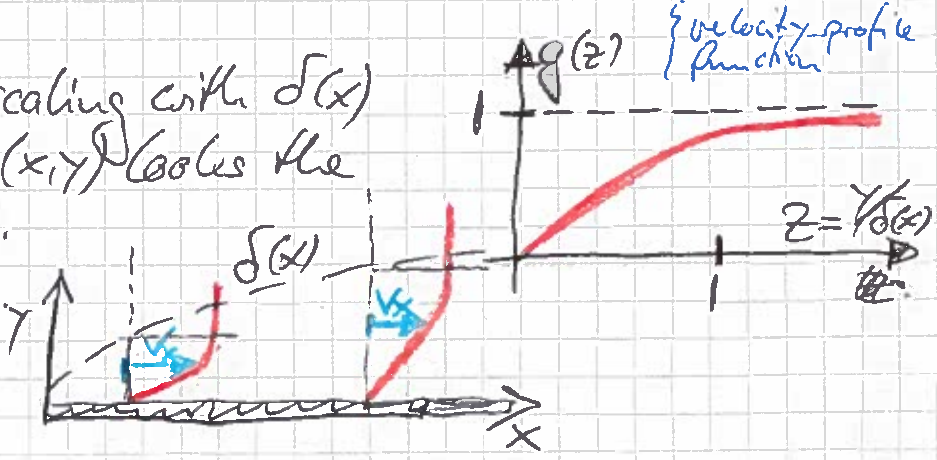
\includegraphics[width=.7\textwidth]{week4/boundary-ansatz}\\
    \caption{Similarity ansatz for the laminar boundary layer.}
    \label{fig:boundary-ansatz}
\end{figure}


\textbf{Question:} does the similarity ansatz work?
\begin{align}
\pdiff{u_x}{x}+\pdiff{u_y}{y} &= 0 \\
\leadsto
u_x = \pdiff{\psi}{y} \ &, \quad u_y = -\pdiff{\psi}{x}
\end{align}

\begin{equation}
\psi(x,y) = u_\infty\delta(x)f\left(\frac{y}{\delta(x)}\right)
\end{equation}

\begin{align}
u_x=\pdiff{\psi}{y} &= u_\infty\delta(x)\diff{f(z)}{z}\diff{z}{y} \\
&= u_\infty \delta(x) \diff{f(z)}{z}\frac{1}{\delta(x)}\\
&= u_\infty \diff{f(z)}{z} \\
&\require u_\infty g(z)
\end{align}

\begin{equation}
f' = \diff{f(z)}{z}g(z)
\end{equation}

\begin{align}
u_y &= -\pdiff{\psi}{x} \\
&=  -u_\infty\diff{\delta(x)}{x}f(z) - u_\infty \delta(x)\diff{f(z)}{z}\diff{z}{x}\\
&= u_\infty \left[-f + \frac{y f'}{\delta}\right] \diff{\delta(x)}{x}
\end{align}

\begin{align}
\pdiff{u_x}{x} &= \left(u_\infty f''\right)\left(\frac{-y}{\delta^2}\right)\diff{\delta(x)}{x} = -\frac{u_\infty y f''}{\delta^2}\diff{\delta(x)}{x} \\
\pdiff{u_x}{y} &= (u_\infty f'') \frac{1}{\delta} = \frac{u_\infty f''}{\delta} \\
\pdiff{u_x}{y} &= \frac{u_\infty f''}{\delta^2}
\end{align}

\begin{align}
\begin{split}
u_x\pdiff{u_x}{x} + u_y\pdiff{u_x}{y} - \frac{\mu}{\rho_0}\ppdiff{u_x}{y} &=
-(u_\infty f') \left(\frac{u_\infty y f''}{\delta^2} \diff{\delta(x)}{x}\right) \\
&\hspace{5mm} + \left(u_\infty\left[-f+\frac{yf'}{\delta}\right]\diff{\delta(x)}{x}\right) \left(\frac{u_\infty f''}{\delta}\right) \\
&\hspace{5mm} -\frac{\mu}{\rho_0} \left(\frac{u_\infty f''}{\delta^2}\right)
\end{split} \\
&= -\frac{u_\infty^2}{\delta}\diff{\delta}{x} ff'' - \frac{\mu}{\rho_0} \frac{u_\infty}{\delta^2}f'''\\
&= 0
\end{align}

\begin{equation}
\frac{\rho_0 u_\infty}{\mu} \delta(x) \diff{\delta(x)}{x} = -\frac{f'''(z)}{f(z)f''(z)} \require c_1^2
\end{equation}

\begin{equation}
\delta\diff{\delta}{x} = \frac{1}{2}\diff{\delta^2}{x} = c_1^2\frac{\mu}{\rho_0u_\infty}\\
\end{equation}

\begin{equation}
\delta^2 = 2c_1^2 \frac{\mu}{\rho_0u_\infty}x + c_2
\end{equation}
$c_2=0$ since $\delta(x=0)=0$.

\begin{equation}
\delta(x) = c_1\sqrt{\frac{2\mu}{\rho_0u_\infty}x}
\end{equation}

\begin{equation}
\delta(x)=\sqrt{\frac{\mu}{\rho_0u_\infty}x}
\end{equation}
Freedom of choice $c_1=\frac{1}{\sqrt{2}}$ because of arbitrary definition of $\delta$; for example, $u_x(y=\delta)=0.99u_\infty$ or $u_x(x=\delta)=0.95u_\infty$.

This is the same result as the order of magnitude calculation when we calculated the x-component of the Navier-stokes equation earlier in this section.

\begin{equation}
f'''(z) +\frac{1}{2} f(z)f''(z) = 0
\end{equation}

\begin{equation}
f(z)\ddiff{f(z)}{z}+2\dddiff{f(z)}{z}=0
\end{equation}
This is Blasius' equation. It is a special case of the more general Falker-Skan equation. The Blasius equation can only be solved numerically. The boundary conditions for the solutions are:
\begin{align}
u_x(y=0)=0&\Rightarrow f'(0)=0, \\
u_y(y=0)=0&\Rightarrow f(0)=0, \\
u_x(y=\infty)=u_\infty&\Rightarrow f'(\infty)=1.
\end{align}
The solution is sketched in \fref{fig:blasius}.
\begin{figure}[!h]
    \centering
    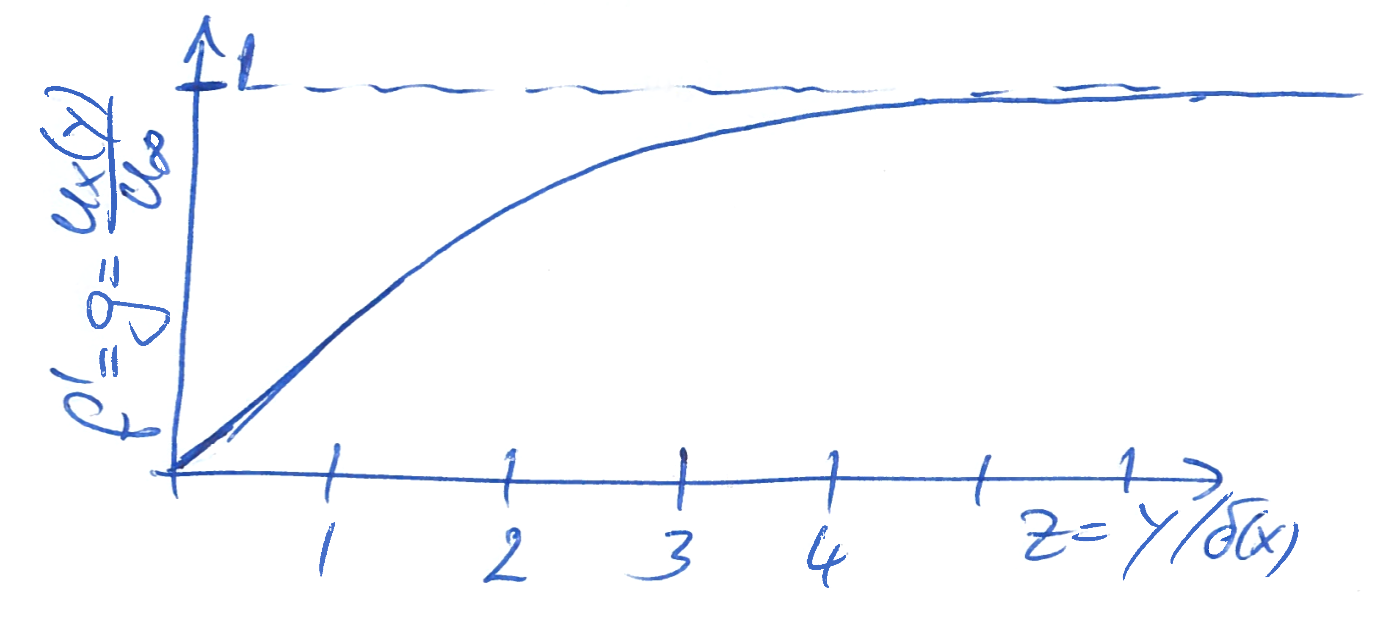
\includegraphics[width=.8\textwidth]{week4/blasius}\\
    \caption{Solution to the Blasius equation.}
    \label{fig:blasius}
\end{figure}


\subsection{Separation of boundary layers}
Boundary condition at the wall:
\begin{equation}
u_x(x,y=0) = u_y(x,y=0)=0
\end{equation}

Prandtl equation (with pressure)
\begin{equation}
u_x\pdiff{u_x}{x}+u_y\pdiff{u_x}{y} = -\frac{1}{\rho_0}\pdiff{p}{x}+\frac{\mu}{\rho_0}\ppdiff{u_x}{y}
\end{equation}
If we are very close to the wall, the two terms on the left side equal zero. We then have
\begin{equation}
\pdiff{p(x,y=0)}{x}=\mu\ppdiff{u_x(x,y=0)}{y}
\end{equation}

\begin{figure}[!h]
    \centering
    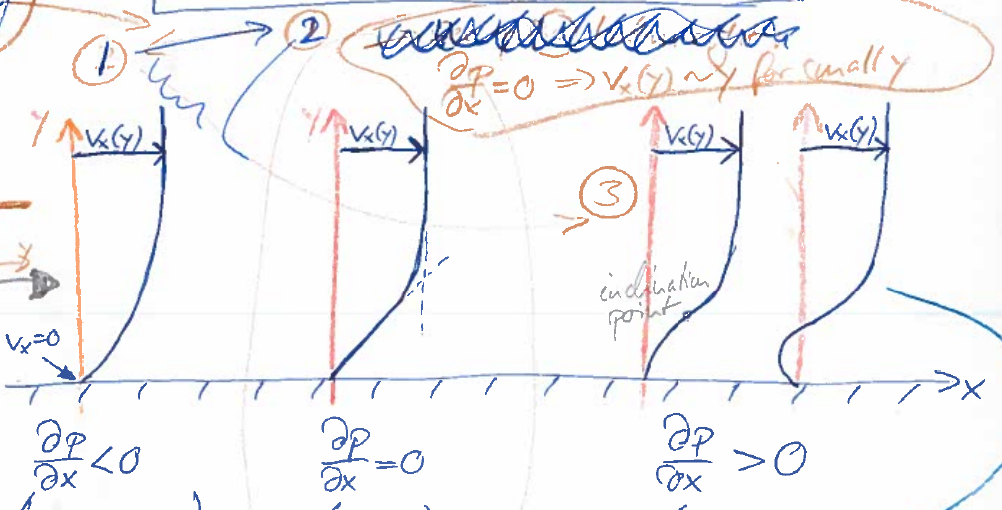
\includegraphics[width=.9\textwidth]{week5/wall-boundary}\\
    \caption{Shape of the boundary layer for different pressure profiles.}
    \label{fig:wall-boundary}
\end{figure}

\begin{figure}[!h]
    \centering
    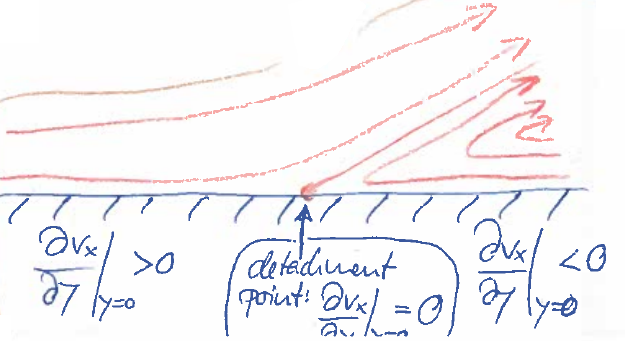
\includegraphics[width=.5\textwidth]{week5/detachment-point}\\
    \caption{Detachment point of the boundary layer.}
    \label{fig:detachment-point}
\end{figure}

\newpage
\textbf{Example:} flow around cylinder

\begin{figure}[!h]
    \centering
    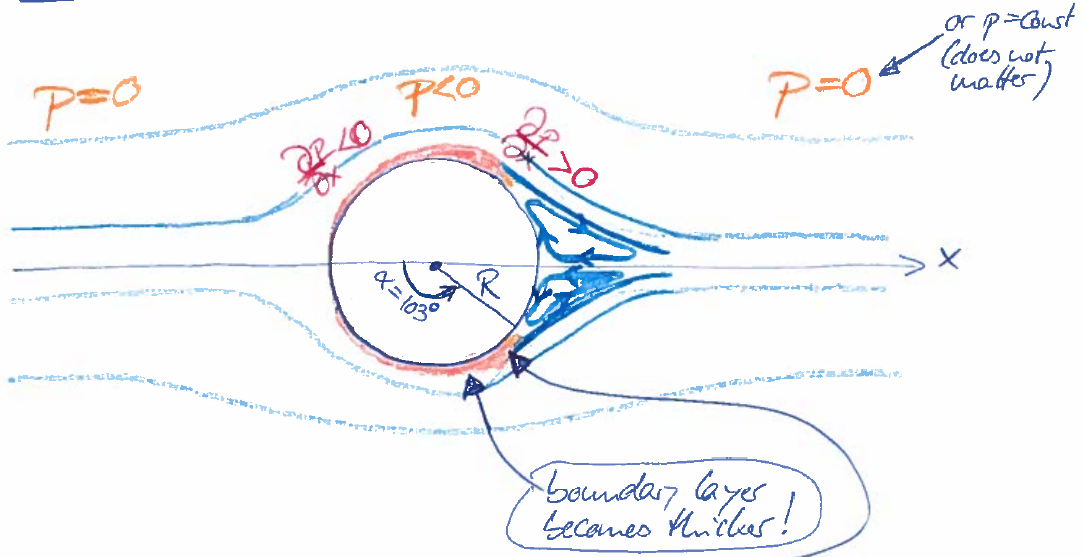
\includegraphics[width=.8\textwidth]{week5/cylinder-flow}\\
    \caption{Separation of boundary layer and detachment point for flow around a cylinder.}
    \label{fig:cylinder-flow}
\end{figure}

The detachment point is at the separation of the boundary layer. When $v\approx0$ there is no kinetic energy to run against the pressure gradient.

\begin{framed}
\textbf{Remark:} separation of boundary layers is a big issue in mechanical engineering; for example: design of airfoils, wind-turbine blades etc.
{\center
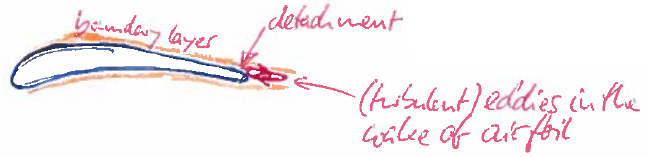
\includegraphics[width=.6\textwidth]{week5/detachment-eddies}\\
}
In case of separation the lift decreases, which can lead to airplane crash. It would also lead to a substantial rise in the overall drag (more friction). This would require more engine power and therefore more fuel for an airplane. For a wind turbine it would means less power generation.

Engineer's dream: construct airfoils without turbulent wake, with e.g. shark skin or fish scales.
\end{framed}


\subsection{Solution of Prandtl equations for free boundary layers}
\fref{fig:2d-laminar-jet} shows a 2-dimensional laminar jet flow generated from a flow through a long slit streaming into a resting fluid.
\begin{figure}[!h]
    \centering
    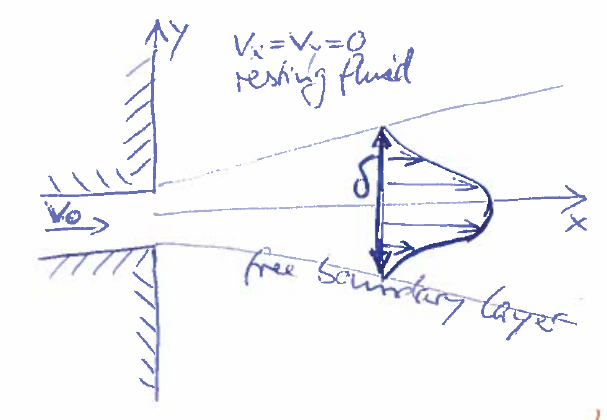
\includegraphics[width=.6\textwidth]{week5/2d-laminar-jet}\\
    \caption{2-dimensional laminar jet flow.}
    \label{fig:2d-laminar-jet}
\end{figure}

We use the Prandtl equations with the similarity ansatz:
\begin{equation}
u_x(x,y)=u_\mathrm{max}(x)g\left(\frac{y}{\delta(x)}\right)
\end{equation}

\begin{equation}
\pdiff{u_x}{x}+\pdiff{u_y}{y}=0 \Rightarrow u_x=\pdiff{\psi}{y},\quad u_y=-\pdiff{\psi}{x}
\end{equation}

\begin{equation}
\psi = u_\mathrm{max}(x)\delta(x)f\left(\frac{y}{\delta(x)}\right)
\end{equation}

\begin{equation}
\pdiff{\psi}{y}=u_\mathrm{max}\delta f'\frac{1}{\delta}=u_\mathrm{max}f'=u_\mathrm{max}g=u_x
\end{equation}

\begin{equation}
u_y=-\pdiff{\psi}{x}=-u'_\mathrm{max}\delta f-u_\mathrm{max}\delta'f-u_\mathrm{max}\delta f'\frac{(-y)\delta'}{\delta^2}
\end{equation}

\begin{align}
\partial_xu_x &= u'_\mathrm{max}f'+u_\mathrm{max}f''\frac{(-y)\delta'}{\delta^2} \\
\partial_yu_x &= u_\mathrm{max} f''\frac{1}{\delta}\\
\partial^2_yu_x &= \frac{u_\mathrm{max}}{\delta^2}f'''
\end{align}
Insertion into Prandtl's equation with $p(x)=\text{constant}$:
\begin{align}
\begin{split}
u_x\partial_x u_x+u_y\partial_yu_x-\frac{\mu}{\rho_0}\partial^2_yu_x &= u_\mathrm{max}f'\left\lbrace u'_\mathrm{max}f' - u_\mathrm{max}\frac{y\delta'}{\delta^2}f''\right\rbrace \\
&\hspace{5mm}-\left\lbrace u'_\mathrm{max}\delta f + u_\mathrm{max}\delta'f-u_\mathrm{max}\frac{y\delta'}{\delta}f'\right\rbrace u_\mathrm{max}\frac{1}{\delta}f'' \\
&\hspace{5mm}-\frac{\mu}{\rho_0^2} \frac{u_\mathrm{max}}{\delta^2}f'''
\end{split}\\
\begin{split}
&= u_\mathrm{max}u'_\mathrm{max}f'^2-u_\mathrm{max}u'_\mathrm{max}ff''-u_\mathrm{max}^2\frac{\delta'}{\delta}ff'' \\
&\hspace{5mm}-\frac{\mu}{\rho_0}\frac{u_\mathrm{max}}{\delta^2}f'''\label{eq:free-boundary}
\end{split} \\
&\require0 \label{eq:prandtl}
\end{align}
All four terms in \eqref{eq:free-boundary} have the form $\alpha_i(x)\beta_i(x)$ for $(i=1,...,4)$. The sum of these four terms has to be zero. This means that $\alpha_1(x)\sim\alpha_2(x)\sim\alpha_3(x)\sim\alpha_4(x)$.

Ansatz:
\begin{align}
u_\mathrm{max}(x) &= c_1x^m\\
\delta(x) &= c_2 x^n
\end{align}

\begin{framed}
\textbf{Remark:} we expect $m<0$ (decreasing velocity with penetration depth) and $n>0$ (increasing thickness of jet with penetration depth).
\end{framed}

Sum of the 4 terms:
\begin{equation}
c_1^2mx^{2m-1}(f'^2-ff'')-c_1^2x^{2m}\frac{n}{x}ff'' - \frac{\mu}{\rho_0}\frac{c_1}{c_2^2}\frac{x^m}{x^{2n}}f'''=0
\end{equation}

\begin{framed}
\begin{equation}
2m-1 = m-2n
\end{equation}
\begin{equation}
m(f'^2-ff'')-nff''-\frac{\mu}{\rho_0}\frac{1}{c_1c_2^2}f'''=0
\end{equation}
\end{framed}

This differential equation determines the velocity profile
\begin{equation}
g\left(\frac{y}{\delta(x)}\right)=f'\left(\frac{y}{\delta(x)}\right)
\end{equation}
of the jet. We are not going to solve this, but we want to know $m$ and $n$, because they determine $u_\mathrm{max}(x)$ and $\delta(x)$. We need a second equation for $m$ and $n$.

\textbf{Second equation:} conservation of momentum flux.
Momentum flux through the red plane in \fref{fig:momentum-flux} is identical to the momentum flux through the blue plane. This means that the integrated momentum flux does not depend on $x$.
\begin{figure}[!h]
    \centering
    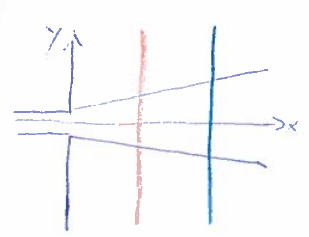
\includegraphics[width=.4\textwidth]{week5/momentum-flux}\\
    \caption{Momentum flux for 2-dimensional laminar jet flow.}
    \label{fig:momentum-flux}
\end{figure}

\begin{align}
\mathrm{momentum} & =\rho_0\Delta V\cdot u_x\\
&= \rho_0\Delta Au_x\Delta tu_x
\end{align}

Momentum flux:
\begin{equation}
\frac{\mathrm{momentum}}{\Delta A \Delta t} = \rho_0 u_x^2
\end{equation}

\begin{framed}
\textbf{Proof of conservation of momentum flux}

If
\begin{equation}
\int_{-\infty}^\infty \rho_0u_x^2(x)dy=\mathrm{constant}
\end{equation}
then
\begin{equation}
\diff{}{x}\int_{-\infty}^\infty \rho_0u_x^2(x)dy=0
\end{equation}

\begin{align}
\diff{}{x}\int_{-\infty}^\infty \rho_0u_x^2(x)dy &= 2\rho_0\int_{-\infty}^\infty\left(u_x\pdiff{u_x}{x}\right)dy \label{eq:a}\\
&= 2\mu\pdiff{u_x}{y}\biggm\vert_{-\infty}^\infty-2\rho_0\int_{-\infty}^\infty u_y\pdiff{u_x}{y}dy \label{eq:b}\\
&=-2\rho_0u_xu_y\biggm\vert_{-\infty}^\infty + 2\rho_0 \int_{-\infty}^\infty\pdiff{u_y}{y}dy \label{eq:c}\\
&= -2\rho_0\int_{-\infty}^\infty u_x\pdiff{u_x}{x}dy \label{eq:d}\\
&= 0
\end{align}
Prandtl's equation \eqref{eq:prandtl} has been inserted into \eqref{eq:a} to obtain \eqref{eq:b}. The first term in \eqref{eq:b} is zero because $u_x(y)=\text{constant}$ for $y\rightarrow\pm\infty$. Partial integration has been used to arrive at \eqref{eq:c}. The incompressibility condition $\partial_xu_x+\partial_yu_y$ has been used to get \eqref{eq:d}. Since \eqref{eq:d} is equal to \eqref{eq:a} the integral has to be zero.
\end{framed}

\begin{align}
\int_{-\infty}^\infty\rho_0u_x^2dy &= \rho_0\int_{-\infty}^\infty u_\mathrm{max}^2(x)g^2\left(\frac{y}{\delta(x)}\right)dy\\
&= \rho_0u_\mathrm{max}^2(x)\delta(x)\int_{-\infty}^\infty g^2(z)dz\\
&\require \mathrm{constant}
\end{align}

\begin{align}
u_\mathrm{max}^2(x)\delta(x)&=\mathrm{constant}\\
c_1^2x^{2m}c_2x^n &= \mathrm{constant}\\
2m+n &= 0
\end{align}

\begin{align}
m+2n=1\ &,\qquad 2m+n=0 \\
\leadsto
m=-\frac{1}{3}\ &,\qquad n=\frac{2}{3}
\end{align}

\begin{align}
u_\mathrm{max}(x)&\sim\frac{1}{x^{1/3}}\\
\delta(x)&\sim x^{2/3}
\end{align}

\begin{framed}
\textbf{Remark:} negative jet flow

Wake behind a wind turbine can be modeled as a negative jet.

{\center
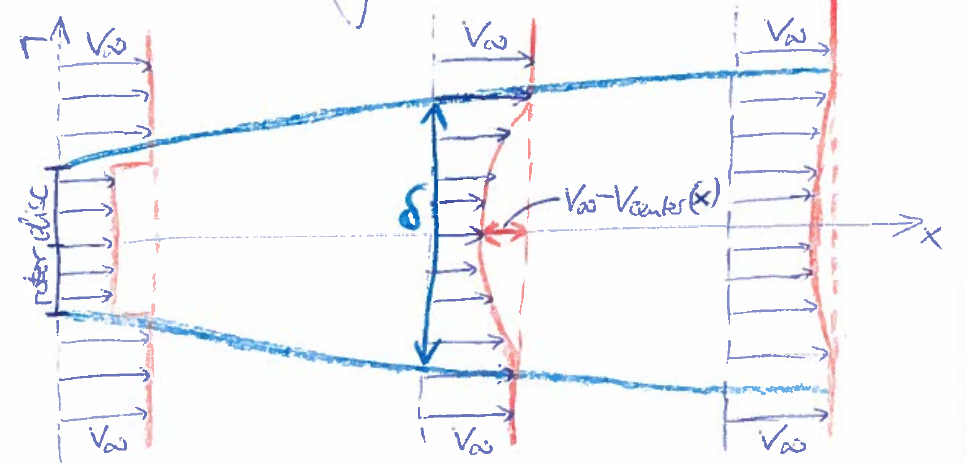
\includegraphics[width=.7\textwidth]{week5/negative-jet}\\
}

\begin{equation}
u_x(x,r) = u_\infty-u_\mathrm{center}(x)g\left(\frac{r}{\delta(x)}\right)
\end{equation}
\end{framed}